\documentclass[10pt,twocolumn,letterpaper]{article}

\usepackage{cvpr}
\usepackage{times}
\usepackage{epsfig}
\usepackage{graphicx}
\usepackage{amsmath}
\usepackage{amssymb}

% Include other packages here, before hyperref.
\usepackage{harmony}
% If you comment hyperref and then uncomment it, you should delete
% egpaper.aux before re-running latex.  (Or just hit 'q' on the first latex
% run, let it finish, and you should be clear).
\usepackage[breaklinks=true,bookmarks=false]{hyperref}

\cvprfinalcopy % *** Uncomment this line for the final submission

%\def\cvprPaperID{****} % *** Enter the CVPR Paper ID here
%\def\httilde{\mbox{\tt\raisebox{-.5ex}{\symbol{126}}}}

% Pages are numbered in submission mode, and unnumbered in camera-ready
%\ifcvprfinal\pagestyle{empty}\fi
\setcounter{page}{1}
\begin{document}

%%%%%%%%% TITLE
\title{Objective evaluation for music generation}

\author{Domenico Stefani\\
\small{mat. 203317}\\
{\tt{\small{domenico.stefani}}\\\tt{\small{@studenti.unitn.it}}}
\and
Matteo Tadiello\\
\small{mat. 207471 }\\
{\tt\small matteo.tadiello\\\tt\small @studenti.unitn.it}
\and
Michele Carbonari\\
\small{mat. 203347}\\
{\tt\small michele.carbonari\\\tt\small @studenti.unitn.it}
}

\maketitle{}
% \thispagestyle{empty}
%%%%%%%%% ABSTRACT

%%%%%%%%% BODY TEXT
\section{Introduction}
Nowadays music generation with deep networks is becoming more and more achievable.
However quality of generated music proved to be hard to evaluate, making subjective evaluation the preferred viable methodology
 of choice.
This entails a series of issues with the \textbf{repeatability} of evaluation results and the \textbf{cost} of such operation.

However, while objective evaluation of creativity in music generation is hard to achieve, evaluation of basic musical metrics and parameters can still be performed rather easily, in order to understand the technical music base on which a set of songs agrees. 


%-------------------------------------------------------------------------
This project is based on the paper \textit{On  the  evaluation  of  generative models in music} \cite{MGeval} that describes possible evaluation metrics to assess properties of music and we used this knowledge to understand the performance of the \textit{Neural Composer} network \cite{Composer}

\section{Generation}

\subsection{Neural Composer}
To generate music we used the \textit{Neural Composer} network which is a classical auto-encoder trained to reproduce 16 measures MIDI files \cite{MidiWiki}. %TODO: find something better than wikipedia
MIDI is the standard music communication protocol that uses codes to describe notes, note intensity and other messages so that a MIDI file can be transcribed as a music score.

\textit{Neural Composer} performs preprocessing on the train songs and encodes each music measure into a 96x96 matrix in which one dimension represents playable notes (96 notes = 8 octaves) and the other represents time.
\begin{figure}[!h]
    \centering
    \[
    A = \begin{bmatrix} 
        a_{11} & a_{12} & \dots \\
        \vdots & \ddots & \\
        a_{K1} &        & a_{KK} 
        \end{bmatrix}
        \]
    \caption{\textit{Where $a_{ij}=1$ means that note i is played at the $\frac{j}{96}$ instant of the current measure}}
\end{figure}

\textit{Neural Composer} consists of a series of 16 encoders applied to 16 measures at a time that have input size 96x96 and 200 output values. The second encoder groups together the 16 vectors of 200 values and reduces this features to 120 latent variables. The latent vector $z$ is then fed into the decoder that mirrors the encoder architecture but employs batch normalization and dropout techniques.

\subsection{Training parameters}
The Composer creator offered an executable synthesizer that used a version of the model trained on 4000 videogame songs for 2000 epochs.
The choice of videogame music is functional to the training phase because this music genre uses rather defined patterns for rhythm and chord progressions.

The first attempts to train the network %ourselves %TODO: keep or remove? maybe too personal the use of 'ourselves' 
proved that these numbers, in conjunction with the specific auto-encoder network, were unsustainable for the Google Colab runtime limits that we worked with, so we decided to reduce the number of tracks and epochs and to compare the metrics on the train set and the generated one, to see how much the performance could possibly degrade under restricted constraints.

\section{Evaluation}


\subsection{Metrics}

\textbf{Pitch-based feature}
\begin{itemize}
    \item \textbf{Pitch count:} The number of different pitches within a samples.
    \item \textbf{Pitch class histogram:} The octave-independent representation of the pitch content plotted in chromatic scale. It  represents the octave-independent chromatic quantization of the frequency continuum.
    \item \textbf{Pitch class transition matrix:} An histogram-like representation of the count of the pitch transition for each pair of notes.
    \item \textbf{Pitch range:} The delta between highest and lowest used pitch in semitones.
    \item \textbf{Average pitch interval:} Average value of the interval between two consecutive pitches in semitones.
\end{itemize}
\textbf{Rhythm-based feature}
\begin{itemize}
    \item \textbf{Note count:} The number of used notes. It not contains pitch information but is a rhythm-related feature.
    \item \textbf{Average inter-onset-interval:} The time between two consecutive notes in the inter-onset-interval in the symbolic domain.
    \item \textbf{Note length transition matrix:} Provides useful information for rhythm description.
    \item \textbf{Note length histogram} Histogram where note length is quantized as the closest length category.
\end{itemize}

\subsection{Train set evaluation}
The first step was to understand what are the characteristics of the music used to train the deep model: for this purpose evaluation have been performed on the train set.

The pitch histogram (Figure \ref{img:train_totalpitchclasshistogram}) shows that a variety of pitches are used but the most common are C,D,E,F,G,A (Do,Re,Mi,Fa,Sol,La) which are part of the C Major scale (Do maggiore), the most common one.
Another interesting insight is that, while there is the possibility of using all possible lengths for notes, videogame music uses mostly Quarter,Eight and Sixteenth notes (\Vier, \Acht, \Sech) which are rather short notes (Figure \ref{img:train_notelengthhist}).



At last, the average number of notes for song is $408.38$ with a high standard deviation that demonstrates that there are fairly complex songs but also songs with very few notes
{(\tt{\textbf{max} total\_used\_note} : 4622.0 \tt{\textbf{min} total\_used\_note} : 9.0)}

\begin{center}
 \begin{tabular}{l r r} 
 \hline
 \textbf{Metric} & \textbf{Mean} & \textbf{Std}   \\ [0.5ex] 
 \hline\hline
 Total used note & 381.96 & 606.83 \\
 \hline
Avg pitch shift & 3.89 & 3.39 \\
 \hline
Note length transition matrix & \multicolumn{2}{r}{Figure.\ref{img:train_notelengthtransitionmatrix} } \\
 \hline
Pitch class transition matrix & \multicolumn{2}{r}{Figure.\ref{img:train_pitchclasstransitionmatrix}} \\
 \hline
Pitch range & 18.71 & 9.69 \\
 \hline
Total pitch class histogram & \multicolumn{2}{r}{Figure.\ref{img:train_totalpitchclasshistogram}}\\
 \hline
Total used pitch & 11.65 & 5.55 \\
 \hline
Note length hist & \multicolumn{2}{r}{Figure.\ref{img:train_notelengthhist}} \\[1ex]
 \hline
\end{tabular}
\end{center}

\subsection{Generated set evaluation}
Once trained the network on over 300 track (for 1000 epochs), 100 songs have been generated and evaluation have been performed on this set.
As can be seen from the evaluation, the generated set has less variability in the \textbf{number of used notes} from sample to sample, and this is due to the fact that the train set contains full length songs, while the Composer network generates only fixed length songs. The pitch shift or \textbf{pitch interval} is the average value of the tonal interval between two consecutive pitches, the fact that it is lower may be a sign that chords have more notes, each one closer to each other, but this value is less informative than other metrics since it requires solid music theory knowledge to understand it. The \textbf{pitch class transition matrices} (Figures \ref{img:train_pitchclasstransitionmatrix} and \ref{img:pitch_class_transition_matrix}) and the \textbf{pitch class histograms} (Figures \ref{img:train_totalpitchclasshistogram} and \ref{img:total_pitch_class_histogram}) instead, show very clear and expected results: the train set contains multiple scales and a discrete amount of variability in the pitch usage, while the generative model uses some pitches with less frequency while focusing on some others.
An unexpected result is that, while the frequency of some notes tend to be lower, the effective range of pitches is unexpectedly larger (on average) than the one from the train set: this may be caused by the presence of very simple short tunes (jingles) in the training set, that uses only a few octaves of the keyboard, while the model tend to be bad at capturing this class of songs.
\subsection{Note length issue}
Finally, the most interesting result is the \textit{note length metrics}: both the  \textbf{Note length transition matrices}  (Figures\ref{img:train_notelengthtransitionmatrix},\ref{img:note_length_transition_matrix}) and the \textbf{note length histograms} (Figures \ref{img:train_notelengthhist} and \ref{img:note_length_hist}) highlight a baffling fact:
\textit{Neural Composer}, under limited training resources, only produces 1/16 notes(\Sech). This may not seem interesting because the sixteenth note was already the most common note in the training set but it is important to remember that the composer is trained on 96x96x16 tensors that deal with each measure with a 96x96 square matrix, to it \textit{should} be agnostic to whether a dimension describes notes or time instants.\\
With the encoding used, the 1/16 note is a submatrix of size [1,6] (1 pitch, 6 time intervals obtained as $\frac{96}{16}$) and this hints that either the model is not agnostic to the note/time difference, or some serious mistakes have been performed in the preprocessing phase.
As much as this seems disappointing for the network, this metrics helped to diagnose a possible issue with some of the ideas or steps in the development of the network itself.

\begin{center}
    \begin{tabular}{l r r} 
        \hline
        \textbf{Metric} & \textbf{Mean} & \textbf{Std}   \\ [0.5ex] 
        \hline\hline
        Total used note & 530.74 & 378.35 \\
        \hline
        Avg pitch shift & 1.97 & 0.99 \\
        \hline
        Note length transition matrix & \multicolumn{2}{r}{Figure.\ref{img:note_length_transition_matrix}} \\
        \hline
        Pitch class transition matrix & \multicolumn{2}{r}{Figure.\ref{img:pitch_class_transition_matrix}} \\
        \hline
        Pitch range & 47.25 & 10.32 \\
        \hline
        Total pitch class histogram & \multicolumn{2}{r}{Figure.\ref{img:total_pitch_class_histogram}} \\
        \hline
        Total used pitch & 27.82 & 12.22 \\
        \hline
        Note length hist & \multicolumn{2}{r}{Figure.\ref{img:note_length_hist}} \\
        \hline
        % avg IOI & 0.04 & 0.04 \\
        % \hline
    \end{tabular}
\end{center}


\section{Conclusions}
In conclusion, it would be interesting to study the music generated by \textit{Neural Composer} trained in optimal conditions, as it seemed much more interesting analyze the capabilities of this network in a complete train condition in order to have a more realistic view of its performances and analyze them from a subjective point.


% TODO: Finish conclusions



{\small
\bibliographystyle{ieee}
\bibliography{egbib}
}



% 
%  Train-related Images
% 

\begin{figure}[!h]
  \centering
  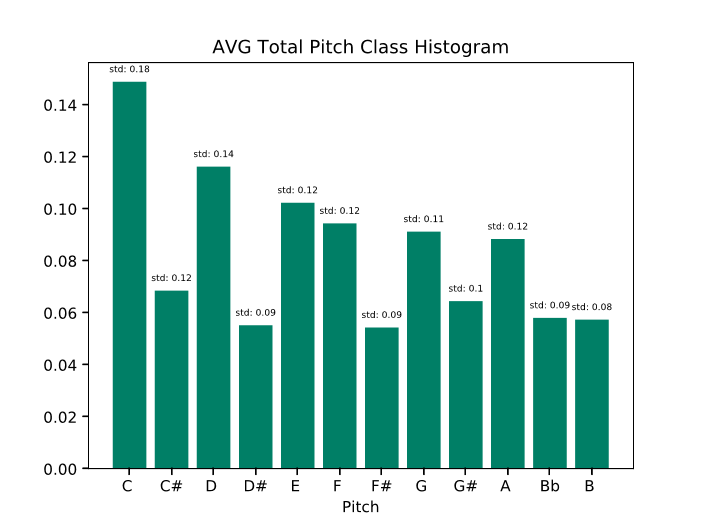
\includegraphics[width = 160pt]{./images/01-abs-train/8.png}
  \caption{Train pitch histogram}
  \label{img:train_totalpitchclasshistogram}
\end{figure}

\begin{figure}[!h]
  \centering
  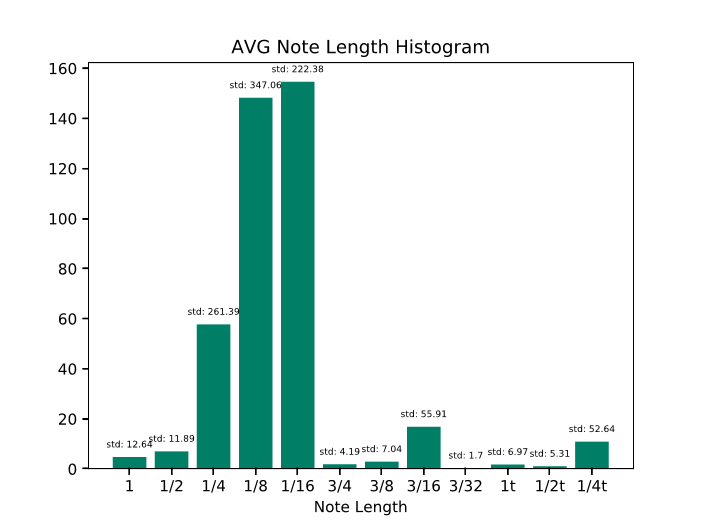
\includegraphics[width = 160pt]{./images/01-abs-train/6.png}
  \caption{Train note length histogram}
  \label{img:train_notelengthhist}
\end{figure}

\begin{figure}[!h]
  \centering
  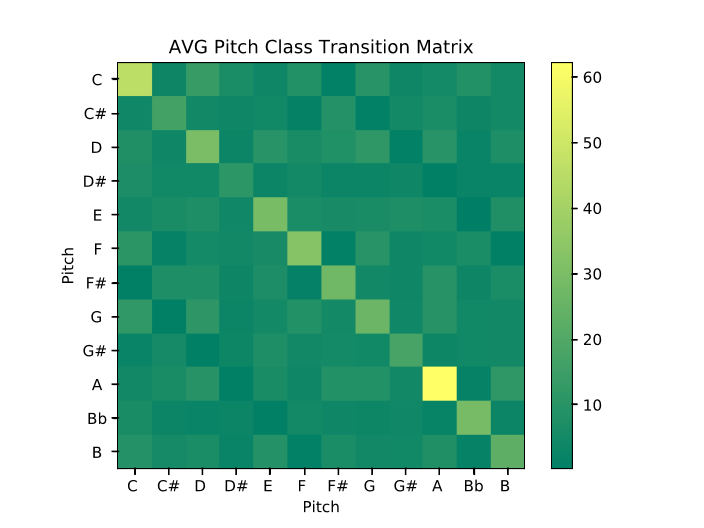
\includegraphics[width = 160pt]{./images/01-abs-train/9.png}
  \caption{Train total pitch class histogram}
  \label{img:train_pitchclasstransitionmatrix}
\end{figure}

\begin{figure}[!h]
  \centering
  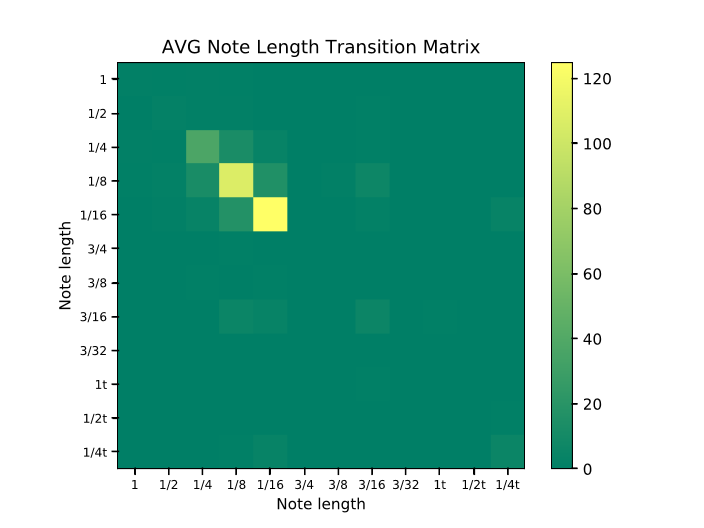
\includegraphics[width = 160pt]{./images/01-abs-train/7.png}
  \caption{Train note length transition matrix}
  \label{img:train_notelengthtransitionmatrix}
\end{figure}


% 
%  Generayrf music Images
% 


\begin{figure}[!h]%[htbp]
  \centering
  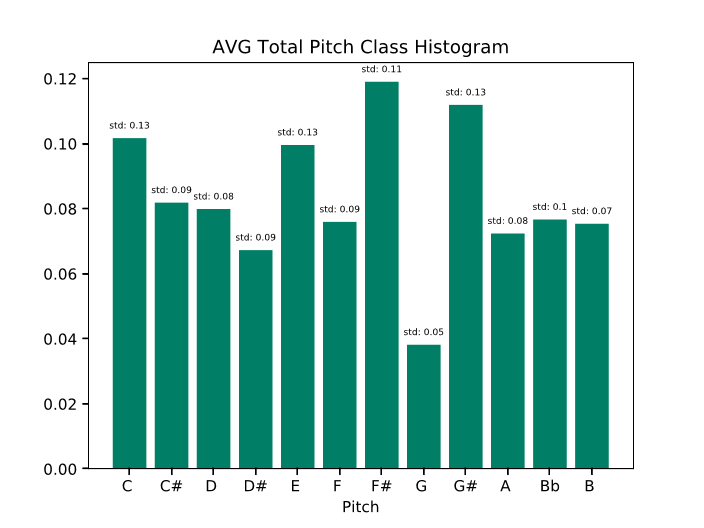
\includegraphics[width = 160pt]{./images/02-abs-gen/8.png}
  \caption{Gen. Total pitch class histogram}
  \label{img:total_pitch_class_histogram}
\end{figure}

\begin{figure}[!h]
  \centering
  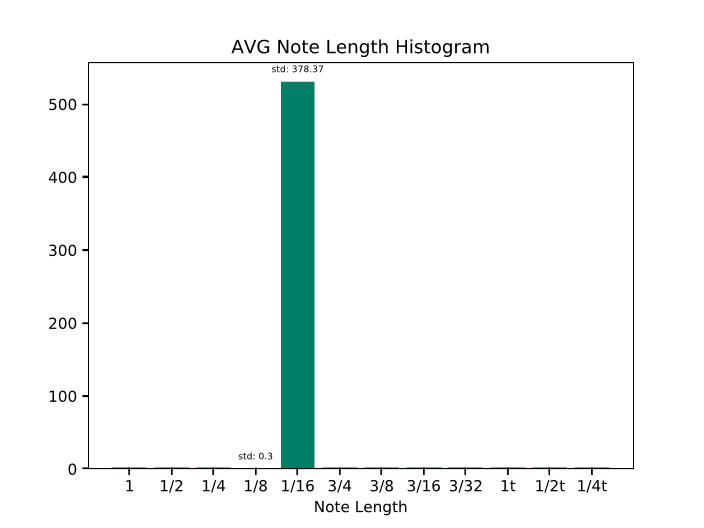
\includegraphics[width = 160pt]{./images/02-abs-gen/6.png}
  \caption{Gen. Note length histogram}
  \label{img:note_length_hist}
\end{figure}

\begin{figure}[!h]
  \centering
  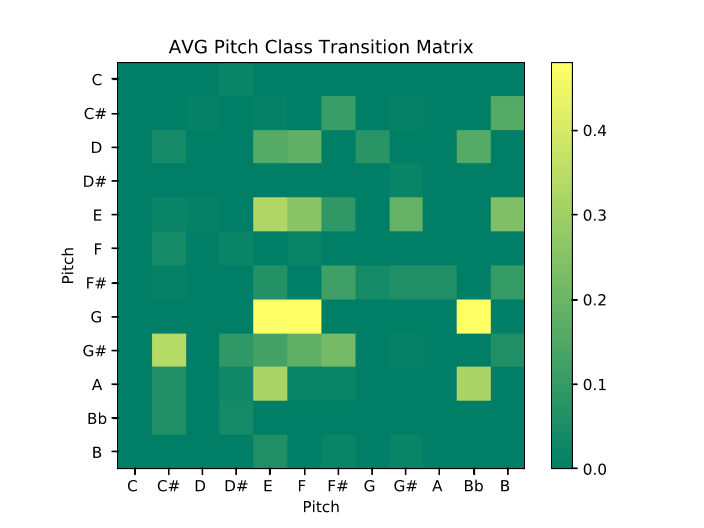
\includegraphics[width = 160pt]{./images/02-abs-gen/9.png}
  \caption{Gen. Pitch class transition matrix}
  \label{img:pitch_class_transition_matrix}
\end{figure}

\begin{figure}[!h]
  \centering
  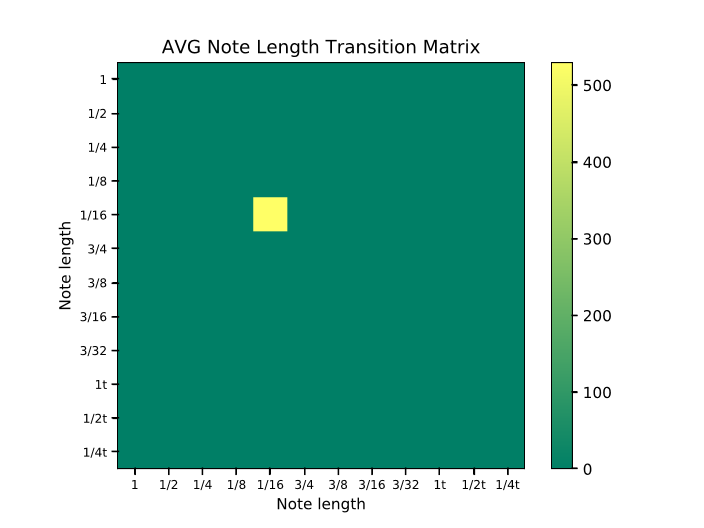
\includegraphics[width = 160pt]{./images/02-abs-gen/7.png}
  \caption{Gen. Note length transition matrix}
  \label{img:note_length_transition_matrix}
\end{figure}



\end{document}
